\documentclass[10pt,a4paper]{article}
\usepackage[utf8]{inputenc}
\usepackage[english]{babel}
\usepackage[T1]{fontenc}
\usepackage{amsmath}
\usepackage{amsfonts}
\usepackage{amssymb}
\usepackage{subcaption}
\usepackage{makeidx}
\usepackage{graphicx}
\usepackage{fourier}
\usepackage{listings}
\usepackage{color}
\usepackage{hyperref}
\usepackage[left=2cm,right=2cm,top=2cm,bottom=2cm]{geometry}
\author{Tommy Müller, Marcus Dittrich, Vincent Noculak}
\title{Zeeman-Effekt}

\lstset{language=C++,
	keywordstyle=\bfseries\color{blue},
	commentstyle=\itshape\color{red},
	stringstyle=\color{green},
	identifierstyle=\bfseries,
	frame=single}
\begin{document}

\maketitle
\newpage
\tableofcontents
\newpage

\section{Theorie}


\subsection{ Einführung}


Unter Zeeman-Effekt versteht man die Aufspaltung von atomaren Spektrallinien unter der Wirkung eines Magnetfeldes. Das äußere Magnetfeld wechselwirkt mit dem magnetischen Moment des Atoms, dadurch werden die Energieniveaus verschoben. Die Verschiebung ist proportional zur magnetischen Flussdichte B. Das Phänomen wurde erstmals 1896 von Pieter Zeeman (1865-1943) beschrieben; 1902 erhielt er dafür den Nobelpreis für Physik. Der Zeeman-Effekt hat große Bedeutung erlangt sowohl in der Astronomie als auch für verschiedene Verfahren der Spektroskopie. So bildet er z.B. die Grundlage der Resonanzmethoden Elektronenspinresonanz (ESR) und kernmagnetische Resonanz (NMR). Der Zeeman-Effekt dient weiterhin zur e/m - Bestimmung sowie zur genauen Ermittlung des Wertes für das Bohrsche Magneton.


\subsection{ Auswahlregeln}


Nicht alle Übergänge zwischen beliebigen Zuständen sind erlaubt. Der Begriff „erlaubt“ ist nicht zu eng zu sehen – verbotene Übergänge können zwar auftreten, sind dann aber deutlich schwächer als die erlaubten, da die hier verwendete Definition [3] vorsieht, dass das Dipolmatrixelement $D_{ik}$  für den Übergang $E_{i}$ → $E_{k}$ ungleich Null $\int <\varphi_{i} |r| \varphi_{k}>\mathrm{d}x$. Verbotene Übergänge können v.a. dann beobachtet werden, wenn – wie hier durch das Magnetfeld – eine äußere Störung erfolgt.   


Generell gelten die Regeln: $ \Delta l=+/-1 ;\Delta m_{l}=\Delta m_{j}= \Delta M_L=0 ,-1,1 \Delta j=0,-1,+1;\Delta s=\Delta S=0;\Delta L=0,-1,1$ Einzige Ausnahme: $\Delta$ j=0 ist nur für j ungleich 0 erlaubt. Diese Regeln lassen sich mit der Drehimpulserhaltung erklären. $\Delta$ S=0 gilt nur für Atome, bei denen die Spin-Bahn-Kopplung schwach ist. Dann kann die Wellenfunktion F  als Produkt der Ortsfunktion Y und Spinfunktion C geschrieben werden. Für das Dipolmatrixelement gilt dann: 
\begin{equation}
D_{ik}= \int\omega_{i}(\overrightarrow{r}_{1},\overrightarrow{r}_{2})r\omega_{k}(\overrightarrow{r}_{1},\overrightarrow{r}_{2})\mathrm{d}x
\end{equation}


für Singulettzustände mit S=0 symmetrisch und andernfalls antisymmetrisch ist, kann $D_{ik}$ nur konstant bleiben, wenn $\Delta$ S=0 gilt.


\subsection{1.3 Polarisation}


Ausgehend vom Dipolmoment kann man zeigen, dass die Polarisation des beim Übergang $E_i$ -> $E_k$  emittierten Lichtes von $D_m$ = $m_{i}$ - $m_{k}$  abhängt. Für $D_{m}$ =  0 ergibt sich linear polarisierte Strahlung, für $D_m$ = − 1 zirkular polarisiertes Licht und analog für $\Delta$m=1 zirkular polarisiertes Licht. Beim normalen Zeeman-Effekt wird die p-Strahlung in Magnetfeldrichtung linear polarisiert, kann also nur senkrecht zum Magnetfeld beobachtet werden und entspricht der Energie der Strahlung ohne anliegendes Magnetfeld. Die anderen beiden Komponenten können aus allen Richtungen beobachtet werden, sind aber entgegengesetzt zirkular in der Ebene senkrecht zum Magnetfeld polarisiert und erscheinen daher für den Betrachter, der senkrecht zur Magnetfeldrichtung beobachtet, linear senkrecht zum Magnetfeld polarisiert.

\subsection{ g-Faktor}

Der Landé-Faktor $g_j$ beschreibt den Zusammenhang zwischen dem Gesamtdrehimpuls $\overrightarrow{j}$ und dem magnetischen Moment:
\begin{equation}
\overrightarrow{\mu}_{j}= \overrightarrow{\mu}_{l}+\overrightarrow{\mu}_{s}=−
\frac {g_{B}}{h}
\overrightarrow{l} + \frac {g_{B}}{h}
\overrightarrow{s}
\end{equation}

mit $g_{s} = 2$ .  Es gilt unter Berücksichtigung des Präzedierens der Vektoren:
\begin{equation}
<\mu_{j}>= \frac {g_{j}\mu_{B}}{h}\overrightarrow{j}
\end{equation}

|j| mit $g_{j}=1+\frac{(j(j+1)+s(s+1)−l(l+1))}{2j(j+1)}$

(Quelle: Demtroeder)
Für das 7$^3S_{1}$ -Niveau von Quecksilber gilt g\textsubscript{j}=2 und für das 6$^3$P\textsubscript{2} -Niveau $g_{j}=\frac{3}{2} $.

\subsection{Normaler Zeeman-Effekt}

Der normale Zeeman-Effekt gilt für S=0 und lässt sich noch anhand eines (halb-)klassischen Modells beschreiben. Dazu wird angenommen, dass sich Elektronen auf festen Kreisbahnen mit Radius r0  um den Atomkern bewegen und einen quantisierten Drehimpuls |$\overrightarrow{L}|=\sqrt{l(l+1)h}$ besitzen.  Einflüsse durch den Spin der Elektronen werden in diesem Modell nicht berücksichtigt.

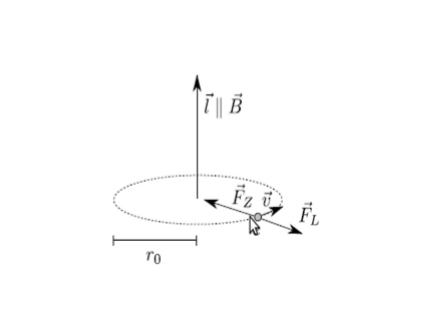
\includegraphics{lotenzmodell}

Abb. 1.1: klassisches Lorentz-Modell mit der Drehbewegung des Elektrons e auf der Kreisbahn (gestrichelt) mit Radius $r_{0}$ und Geschwindigkeit $\overrightarrow{v}$ , sodass sich der Drehimpuls $\overrightarrow{l}$ und die Zentrifugalkraft $\overrightarrow{F}_{Z}$ ausbilden sowie – bei angelegtem Magnetfeld ⃗$\overrightarrow{B}$ – die Lorentz-Kraft ⃗$\overrightarrow{F}_{L}$ einstellt.\\


Nimmt man an, dass die Drehbewegung wie in Abb. (1.1) in der x-y-Ebene stattfindet und der Drehimpulsvektor also senkrecht auf dieser steht, so ergeben sich mit der Zentrifugalkraft
und der Lorentz -Kraft für das Magnetfeld $\overrightarrow{B}=B_{Z}$ die Bewegungsgleichung


\begin{align}
m_{e}\ddot x=−m_{e}\omega_{0}^2 x+e\dot{y}B m_{e}\\
m_{e}\ddot y=−m_{e}\omega_{0}^2 y+e\dot{x}B\\
m\ddot z=0 
\end{align}


wobei noch $r_{0}=\sqrt (x^2+y^2)$ gilt. Die Annahme $\overrightarrow{l}|| \overrightarrow{B}$  ist zulässig, weil sich der Drehimpuls immer nach dem Magnetfeld ausrichten wird. Die Lösung dieser gekoppelten inhomogenen Differentialgleichung ist eine Überlagerung gegenläufiger Rotationen mit $w_{0}= \mp w_{L}$ , wobei die Larmor -Frequenz $w_{L} = \frac{eB}{2m_{e}}$ beträgt. Mit einer neuen Koordinate x' lässt sich die Bewegungsgleichung schreiben als: x'=C e$^{i(w_{o}-w_{L})t}$+$D e^{i(w_{o}+w_{L})t}$
\\


Wenn die Bahngeschwindigkeit erhalten bleiben soll,  gibt es drei Möglichkeiten: ist C=0 aber D ungleich 0 , so ergibt sich eine Rotation mit der Energie $E_{a}=\hbar (w_{o}+w_{L})$ und bei dem symmetrischen Fall D=0 und C ungleich 0 erhält man $E_{b}=\hbar(w_{o}$-$w_{L})$ . Die dritte Variante ist C=D . Damit gilt:  x'=C e$^{i(w_{o}-w_{L})t}$+D e$^{i(w_{o}+w_{L})t}$ = Ce$^{i(w_{o}t}$ und daher E=$\hbar w_{0}$ . Es gibt also eine Aufspaltung der Energien in drei Niveaus, deren Frequenzabstand Δv=
$\mu_{B} \hbar$ mit dem 
Bohrschen Magneton $\mu_B$  beträgt. Da der Drehimpuls ⃗$\overrightarrow{L}$ und insbesondere dessen z Komponente $l_z=m\hbar$  quantisiert ist, können nur ganzzahlige Vielfache von $\hbar$  auf die Strahlung übertragen werden. Nach den Auswahlregeln gilt jedoch Δm=0,$\pm$1 , sodass man mit $\Delta$m=0 Licht mit dem Drehimpuls 0 – also linear polarisiertes Licht – erwartet und ansonsten zwei Komponenten mit entgegengesetzt zirkular polarisiertem Licht erwartet werden, deren Drehimpuls $\pm\hbar$  beträgt. Eine alternative Erklärung lässt sich über das magnetische Moment ⃗$\overrightarrow{\mu}_M$  einführen. Die zusätzliche potentielle Energie in einem Magnetfeld lautet dann: $\Delta E_{pot}$=−$ ⃗\mu_M B$\\


Mit der Nomenklatur aus Abb. (1.1) ergibt sich: $\mu_M|=I⋅2\pi r_0^2=−evr/2$ und für den Drehimpuls$ |⃗\overrightarrow{l}|=mer_0v$ Beide Vektoren sind parallel zur Drehachse, also gilt:$\mu_m=− e 2me ⋅⃗\overrightarrow{l}$ Mit einem nur in z -Richtung wirkenden Magnetfeld gilt für die z -Komponente des Drehimpulses ⃗$\overrightarrow{\mu}_m⃗\overrightarrow{e}_z$=−$\frac{e}{2m_e}$ ⋅m$\hbar$ Damit gilt für die Energiedifferenz zwischen zwei Energieniveaus, die sich um $\Delta m=|m_1-m_2|$ unterscheiden  $\Delta E_{pot}=\mu_B\Delta m$ Insgesamt ergeben sich so 2l+1 mögliche Energieniveaus. Der Übergang der grünen Linie bei 546,07 nm erfolgt nach Tab.(1) von $7^3S_1  zu 6^3P_2$. Damit ergibt sich das Schema in Abb.(1.2)

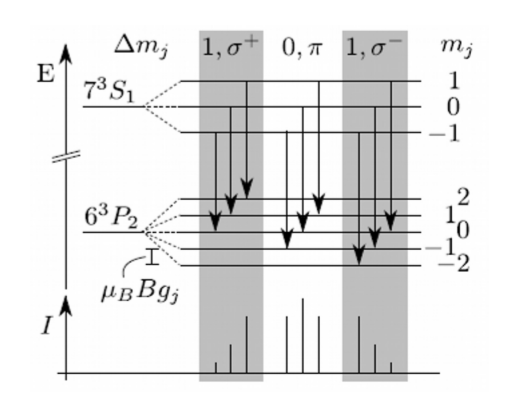
\includegraphics{73s1}

Abb.1.2: Termschema der Zeeman-Aufspaltung mit dazugehörigen Intensitäten der Linien für die grüne Quecksilber-Linie im Magnetfeld nach [3, 4, 9]; die unterschiedlichen Abstände der Linien sind auf die verschiedenen $g_j$ zurückzuführen

\subsection {Anomaler Zeeman-Effekt}


Betrachtet man den gegenüber dem normalen Zeeman-Effekt verallgemeinerten Fall von Zuständen mit S ungleich 0 , so ergibt sich der nur quantenmechanisch erklärbare anomale Zeeman-Effekt. Zwar bleibt der aus der Spin-Bahn-Kopplung resultierende Gesamtdrehimpuls
⃗$\overrightarrow{j}=⃗\overrightarrow{l}+⃗\overrightarrow{s}$ auch im äußeren Magnetfeld dem Betrag nach erhalten, allerdings präzediert er um die z-Achse, weil das Magnetfeld ein Drehmoment ausübt.

$\overrightarrow{j}$  und ⃗$\overrightarrow{\mu}μ_j$ sind nicht mehr parallel; ⃗$\overrightarrow{\mu}_j$  präzediert um den Erwartungswert < ⃗$\overrightarrow{\mu}_j$> , der sich aus der Projektion von ⃗$\overrightarrow{\mu}_j$  auf ⃗$\overrightarrow{j}$  ergibt: <$ ⃗\overrightarrow{\mu}_j$>=$\frac{\overrightarrow{\mu}_j\overrightarrow{j}}{\overrightarrow{|⃗j|}$} =−$\frac{e}{2m_e}$ ⋅($ \frac{\overrightarrow{l}\overrightarrow{j}} {|⃗\overrightarrow{j}|}$ + $\frac{ g_s⃗\overrightarrow s \overrightarrow j}{|⃗\overrightarrow j|}$ )

Durch Quadrieren von Umformungen können die Skalarprodukte ersetzt werden: ⃗

$\overrightarrow{l} \overrightarrow{j} =\frac{\hbar^2}{ 2} $⋅(j(j+1)+l(l+1)−s(s+1))

$ ⃗\overrightarrow{s} \overrightarrow{j}=\frac {\hbar^2} {2}$ ⋅(j(j+1)−l(l+1)+s(s+1))

Damit ergibt sich  
\begin{equation}
<\mu_j>=−m_jg_j\mu_B 
\end{equation}
sodass die Energieaufspaltung zwischen zwei Energieniveaus mit $\Delta m=|m_1−m_2|  $

\begin{equation}
\Delta E_{pot}=g_j\mu_B B\Delta m
\end{equation}

beträgt.

\textbf{Frequenzauspaltung(Aufgabe 5.9):}
Die Messgleichung setzt an der Gleichung zur Bestimmung der Brennweite an. Da folgendes gilt:

$\lambda =2d(1- \frac{r^2}{2f^2})$

$ ((\lambda+\Delta\lambda)2d(1-\frac{R^2}{2f^2}))=

\lambda*2d(1-\frac{r^2}{2f^2}))$$\Delta\lambda(1−(R)^2/(2f^2))

= \frac {\lambda} {2f^2}$$ ((R)^2-r^2) $
mit\\
$ \frac {R^2} {2f^2} = 0 $ für R<<f gilt:

\begin{equation}
\Delta \lambda =\frac {\lambda (R^2 -r^2)} {2f^2}
\label{1v}
\end{equation}
Daraus ergibt sich die Frequenzverschiebung 


$\Delta v=\frac{c}{\lambda}  -\frac{c}{\lambda+\delta\lambda}$ =


\begin{equation}
\Delta v = \frac {c*\Delta \lambda} {\lambda^2}
 \label{1f}
\end{equation}


woraus wir wiederum die Energieverschiebung errechnen können. 

$\Delta E=\hbar \Delta v$

\subsection{ Fabry-Pérot-Interferometer} 

Das Interferometer besteht aus zwei planparallelen Platten, deren Oberflächen jeweils teilverspiegelt sind, sodass ein Teil der einfallenden Strahlung durchgelassen wird und somit auch einen Teil der Wellenfront bildet, während der Rest wieder zurück in das Spalt reflektiert wird. Vor diesem optischen Resonator befindet sich ein Mikroskopaufbau, sodass die Objektivbrennweite bei der Justierung des Aufbaus zu berücksichtigen ist. Von der Strahlungsquelle aus betrachtet, findet sich zunächst eine Sammellinse, die aus der Punktlichtquelle annähernd eine Flächenlichtquelle macht und hinter der sich ein Kollimator befindet. Der Abstand zwischen diesen beiden Linsen muss der Brennweite der Kollimatorlinse entsprechen. Im Okular sind dann konzentrische Ringe zu beobachten, die HAIDINGERsche Ringe genannt werden. Um auf diese Weise mehrere versetzte Strahlengänge zu erhalten, ist der Anteil der reflektierten Strahlen recht groß. Durch den über das gesamte Material konstanten Oberflächenabstand d und den Einfallswinkel a in Bezug auf die Flächennormale kann somit der Abstand der jeweiligen Wellenbündel und damit die Weglängendifferenz d festgelegt werden.


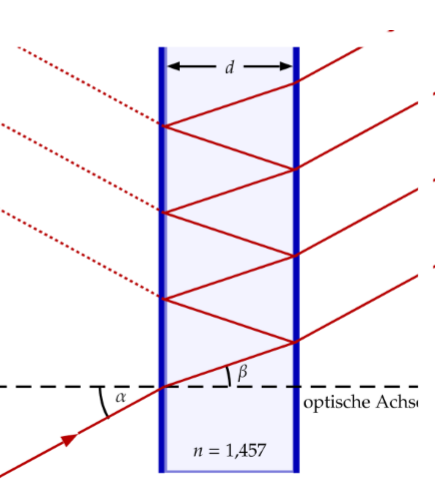
\includegraphics{fab}

Abb. 1.3 Strahlengang im Fabry-Perot-Etalon (Quelle: semibyte.de)


Die Bedingung für konstruktive Interferenz ist erfüllt, wenn die Weglängendifferenz des Lichts $\Delta$ s ein Vielfaches der Wellenlänge Lambda ist.\\

$\Delta s=m\lambda$=2nd$\cos(\alpha)$\\

$\lambda= \frag{2ndcos(\alpha)}/ {m} $\\

Das Spektrometer arbeitet mit divergentem einfallendem Licht und einer Linse, um das Interferenzmuster auf eine Platte zu projektieren. Das entstehende Bild besteht aus konzentrischen Kreisen. 
Die Interferenzbedingung lautet z=(2d/$\lambda$ )∗(1 -$\frac{r^2} {2f^2} )$ , wobei f die Brennweite, r der Radius des beobachteten Kreises ist. Der Einfallswinkel wurde angenähert, sodass in die Formel noch die Taylorentwicklung cos(α)=1-$\alpha^2$/ 2 miteingeht.

\subsection{ Gittermonochromator}

Obwohl bereits das Fabry-Perot-Interferometer als Monochromator wirkt, so hilft das vorgeschaltete Gitter zur Auswahl des gewünschten Spektralbereichs. Durch das Drehen des Gitters ändert sich der Spektralbereich, für den das Gerät durchlässig ist. Dieser Bereich ist verglichen mit dem des Interferometers groß und kann durch zusätzliche Blenden vor den Spiegeln verkleinert werden, sodass das Auflösungsvermögen auf Kosten der Intensität steigt. 

Das polychromatische Licht tritt durch den Eingangsspalt und fällt auf einen konkaven Spiegel. Es wird ein paralleler Strahl erzeugt. Das Gitter zerlegt durch Beugung diesen Strahl in einzelne Wellenlängen. Ein zweiter konkaver Spiegel bündelt das zerlegte Licht auf der Brennebene. Die Stellung des Gitters bestimmt die Wellenlänge, die durch den Ausgangsspalt in der Brennebene durchgelassen wird. Reflexionsgitter sind verbreiteter als Transmissionsgitter.

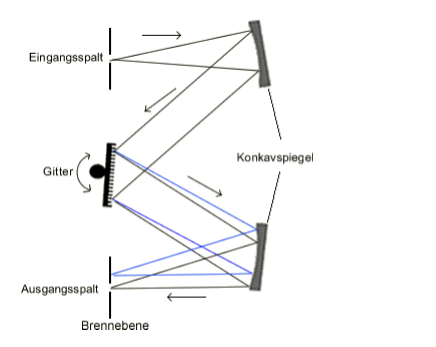
\includegraphics{gitter}

Abbildung 1.4 schematischer Aufbau eines Gittermonochromators (Quelle: chemgapedia.de)

\section{Durchführung}

In dem Versuch sollte der normale Zeeman-Effekt beobachtet werden. Abbildung \ref{aufbau} zeigt den Aufbau des Versuchs. Mit Hilfe einer Quecksilber-Spektrallampe, die sich für Teile der Messung in einem Magnetfeld befindet, wird Licht erzeugt. Dieses wird durch eine Sammellinse gebündelt und durch einen Monochromator geleitet, mit dessen Hilfe bestimmte Spektrallinien des Lichts gezielt durchgelassen werden können. Das vom Monochromator durchgelassene Licht läuft dann durch eine Linse, gefolgt von einem Fabry-Perot-Interferometer. Durch eine Kamera kann das Licht nach dem Fabry-Perot-Interferometer am Computer untersucht werden. 

Der Versuch begann damit, das Spektrum der Quecksilber-Spektrallampe bei noch ausgeschaltetem Magnetfeld mit Hilfe des Monochromators zu beobachten. Daraufhin wurde unter Beobachtung der grünen Spektrallinie der Strahlengang auf optimale Schärfe justiert. Hierzu wurden die vom Fabry-Perot-Interferometer erzeugten Ringe betrachtet und darauf hin aufgenommen.

Jetzt wurde das Magnetfeld angeschaltet, um den normalen Zeeman-Effekt zu untersuchen. Ausgehend von der grünen Spektrallinie, wurde die Polarisation der Zeeman-Komponenten und die Aufspaltung der Spektrallinie abhängig von der Stärke des Magnetfelds beobachtet.

\begin{figure}[h]
	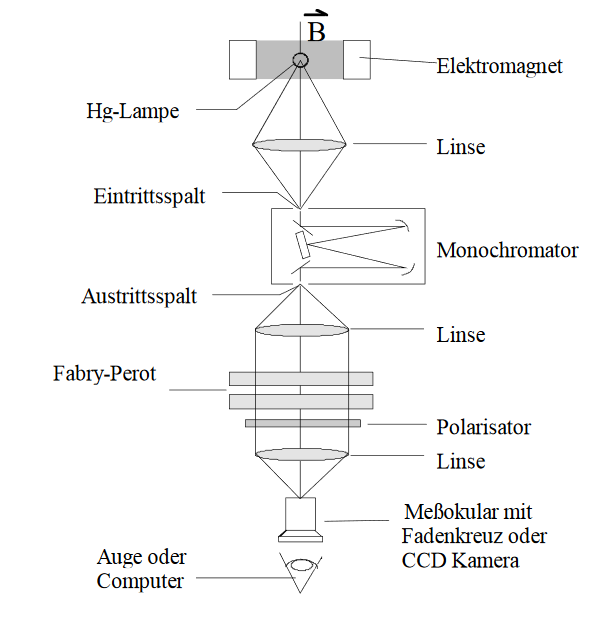
\includegraphics[scale = 1]{Zeeman_aufbau.png}
	\centering
	\caption{Versuchsaufbau, Quelle: Versuchsanleitung vom Zeeman-Effekt-Versuch des Fortgeschrittenenpraktikums}
	\label{aufbau}
\end{figure}

\section{Versuchsauswertung}


Mit dem Monochromator hatten wir zum Beginn des Versuchs das Feinstrukturspektrum der Quecksilber-Spektrallampe von $400nm$
bis $900nm$ beobachtet. An dem Monochromator konnte per Rad die durchgelassene Wellenlänge eingestellt werden. Eine Angabe zu der Durchlassgenauigkeit des Monochromators konnten wir nicht finden. In Tabelle \ref{spektrum} können die von uns beobachteten Spektralfarben gesehen werden. Wir waren in der Lage, die meisten Spektralfarben mit einer Abweichung von höchstens 4 Nanometern wahrzunehmen. Die cyanfarbige und rote Spektrallinie konnten wir nicht beobachten. Es fällt auf, dass die von uns beobachteten Spektrallinien immer ein paar Nanometer über den tatsächlichen Literaturwerten gemessen worden sind. Dies könnten an einem systematischen Fehler am Monochromator liegen.

Die bei $577nm$ und $579nm$ liegenden orangenen Spektrallinien der Spektrallampe konnten wir nur als einzelne Linie bei $580nm$ wahrnehmen.



\begin{table}[h!]
	\centering
\begin{tabular}{|l|r|c|lrp{16cm}}\hline
	Farbe & Literaturwerte in nm & Beobachtete Wellenlängen in nm\\\hline
	Violett & 405 & 409\\
	Blau & 436 & 439\\
	Cyan & 492 & -\\
	Grün & 546 & 548\\
	Orange & 577 & 580\\
	Orange & 579 & 580\\
	Rot & 615 & -\\\hline
\end{tabular}
	\caption{Beobachtete Spektrallinien der Quecksilber-Spektrallampe}
	\label{spektrum}
	
	
\end{table}\\\\
\\
\\
\subsection {Bestimmung der Radien der Interferenzordnung}

Wir hatten den Versuchsaufbau auf die grüne Linie des Spektrums optimiert. Wir nahmen kein Spalt da die Intensität sich zu sehr verringerte. Die Radien haben wir an der grünen Linie gemessen, die wir bei 548 nm gemessen haben. Es gelang uns den Radius der ersten 7 Ordnungen zu bestimmen. Die Längenangabe auf dem Bildschirm war 1 Pixel mit 4,65 µm. Den Nulldurchgang haben wir bei 286 Pixel lokalisiert. Mit dem Programm Peak o Mat haben wir dann die einzelnen Peaks den Radien zugeordnet. Mit diesen Daten ( Peaks und Wellenlänge ) konnten wir dann die Brennweite bestimmen.\\
\\
Ordnung 1 - 508 Pixel\\
Ordnung 2 - 614 Pixel\\
Ordnung 3 - 693 Pixel\\
Ordnung 4 - 759 Pixel\\
Ordnung 5 - 817 Pixel\\
Ordnung 6 - 869 Pixel\\
Ordnung 7 - 917 Pixel\\
\\
Mit der Formel für die Brennweite haben wir zu jeder Ordnung den Wert ausgerechnet und den Mittelwert der Brennweiten genommen, Fehler war der größte Abstand vom Mittelwert zu den Ordnungen. \\
Mittelwert: f = 109,8 $\pm$ 18,7


\subsection{Bestimmung der Frequenzaufspaltung}

%Die Nummer der Formel muss noch hinzugefügt werden
Die Frequenzaufspaltung durch das Magnetfeld kann mit Hilfe von Formel \ref{1v}und\ref{1f}	 Bestimmt werden. Der dazugehörige Fehler lässt sich mit den Gesetzen der Fehlerfortpflanzung als folgenden bestimmen:

\begin{equation}
\Delta\Delta\nu = \frac{c}{\lambda} \sqrt{(\frac{r_1}{f^2} \cdot\Delta r_1)^2 + (\frac{-r_2}{f^2}\cdot \Delta r_2)^2 + (\frac{r_1^2 - r_2^2}{f^3} \cdot \Delta f)^2)}
\label{fehler123}
\end{equation}
 Wir haben die Aufspaltung des grünen Lichts der Spektrallampe gemessen. Aus Tabelle \ref{spektrum} kann abgelesen werden, dass das grüne Licht eine Wellenlänge von $546 nm$ hat. Die Brennweite der verwendeten Linse, die wir zur Berechnung der Frequenzaufspaltung benötigen, haben wir schon berechnet.
%, sie beträgt...
Die Zeeman-Aufspaltung $\Delta\nu$ einer Spektrallinie ist nach oben die gleiche, wie nach unten. Deshalb können wir zur Berechnung der Aufspaltung den Ring im Interferometer mit kleinerem und höherem Radius nehmen(Von den 3 Ringen gleicher Ordnung) und zum Schluss die damit berechnete Frequenzaufspaltung durch 2 teilen. Den jeweils dritten Ring mit durch den Zeeman-Effekt unverändertem Radius müssen wir nicht beachten. Wir benutzen bei den verschiedenen Magnetfeldstärken jeweils die Radien der Ringe der ersten Ordnung. 
Mithilfe der vorgegebenen Eichkurve aus der Versuchsanleitung können die zu unseren gemessenen Strömen zugehörige Magnetfelder bestimmt werden. (Tabelle \ref{gemessene_frequenzaufspaltungen}).

Der Zusammenhang zwischen der Frequenzaufspaltung und der Wellenzahlaufspaltung durch den Zeeman-Effekt ist gegeben durch $\Delta k = \frac{2 \cdot \pi}{c} \cdot \Delta\nu$.

Die berechnete Frequenzaufspaltung in GHz und $cm^{-1}$ können in Tabelle \ref{gemessene_frequenzaufspaltungen} gesehen werden.
%Ergebnis kommentieren

Da wir nun Messergebnisse der Frequenzaufspaltungen für verschieden starke Magnetfelder haben, können wir diese gegenüber in einem Diagramm Auftragen. Die Ausgleichsgeraden, sowie die Grenzgeraden wurden mithilfe linearer Regression berechnet. Hier hat die obere Grenzgrade die Steigung $b + \Delta b$ und schneidet die y-Achse bei $a + \Delta a$ und die untere Grenzgerade hat die Steigung $b - \Delta b$ und schneidet die y-Achse bei $a - \Delta a$. Die berechneten Werte für $b$, $\Delta b$, $a$ und $\Delta a$ können in Tabelle \ref{diagramm_werte} gesehen werden.
 Wir betrachten ein Diagramm von $\Delta\nu$ gegen $B$ in \ref{diagramm_aufspaltung} und eins von $\Delta k$ gegen $B$. Weil sich $\nu$ und $k$ nur um einen Vorfaktor unterscheiden, reicht es, wenn wir nur \ref{diagramm_aufspaltung} betrachten.
Weil die Frequenzaufspaltung des Zeeman-Effekts proportional zu $B$ ist, sollte bei einer perfekten Messung die Gerade durch den Koordinatenursprung gehen.




\begin{figure}[h]
	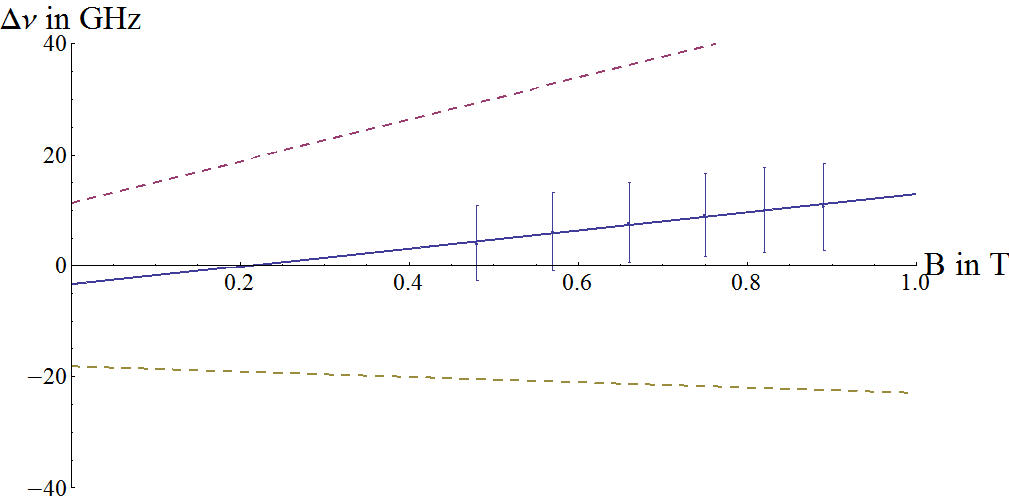
\includegraphics[scale = 0.5]{frequenzaufspaltung.png}
	\centering
	\caption{Durch den Zeeman-Effekt hervorgerufene Frequenzaufspaltung, abhängig vom Magnetfeld}
	\label{diagramm_aufspaltung}
\end{figure}
\begin{figure}[h]
	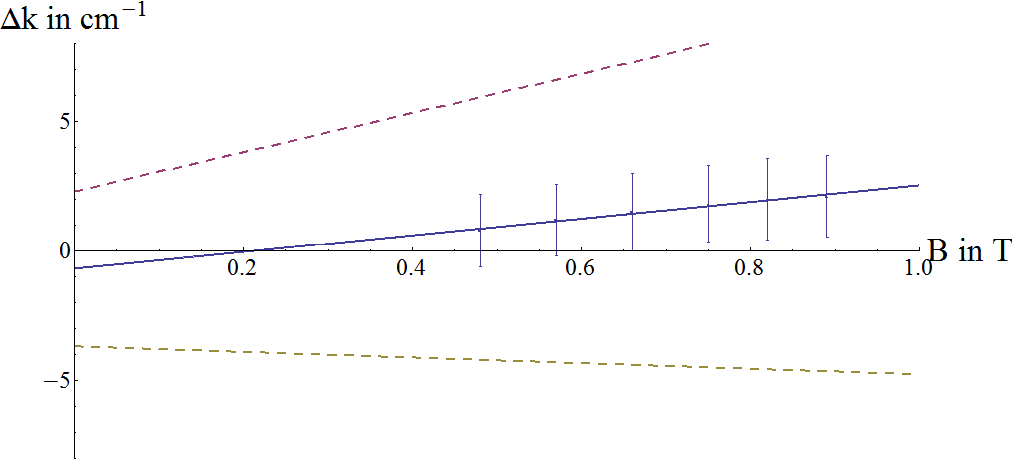
\includegraphics[scale = 0.5]{wellenzahlaufspaltung.png}
	\centering
	\caption{Durch den Zeeman-Effekt hervorgerufene Wellenzahlaufspaltung, abhängig vom Magnetfeld}
	\label{diagramm_aufspaltung_wellenzahl}
\end{figure}


\begin{table}[h!]
	\centering
	\begin{tabular}{|l|r|c|lrp{16cm}}\hline
		Steigung in $\frac{GHz}{T}$ & a in $GHz$\\\hline
		$15 \pm 20$ & $-3 \pm 14$\\\hline
	\end{tabular}
	\caption{Steigung b und Achsenabschnitt a  des Diagramms $\Delta\nu$ gegen $B$}
	\label{diagramm_werte}
\end{table}



Die durch den Zeeman-Effekt hervorgerufene Energiedifferenz zwischen zwei Atomzuständen mit gleicher Haupt- und Nebenquantenzahl ist gegeben durch

\begin{align}
	E_{mj+1}- E_{mj} = \Delta E_{Zeeman} = g_j \mu_B B \\
	\Rightarrow h \Delta \nu =  g_j \mu_B B \\
	\Rightarrow \Delta \nu = \frac{g_j \mu_B}{h} B
	\label{steigungnu}
\end{align}

\section{Messung der Zeeman Aufspaltung}
\\

\subsection{Grüne Linie}
\\
Wie schon in der theoretischen Vorbereitung besprochen, führt ein angelegtes Magnetfeld zu einer Aufspaltung diskreter Energieniveauübergänge, was zu einer Aufspaltung der Spektrallinien führt. Durch Beobachtung der Photonen transversal zum Magnetfeld lässt sich das Licht in zwei Komponenten aufteilen. Die sogenannte $\pi - $ Komponente ist linear und parallel zur Richtung des Magnetfeldes polarisiert und energetisch, in Bezug auf die Frequenz ohne Magnetfeld, nicht verschoben. Die sogenannte Sigma-Komponente ist zirkular und senkrecht zur Richtung des Magnetfeldes polarisiert. Die Sigma-Komponente liefert zwei Spektralkomponenten ($\sigma _{-}$, $\sigma _{+}$), welche in der Frequenzbetrachtung der Photonen, $\pm $ um   die Lamorfrequenz zur $\pi - $ Komponente verschoben sind.  
\\
\begin{figure}[h]
	\includegraphics[scale = 1]{Zeeman_splitting.png}
	\centering
	\caption{Versuchsaufbau, Quelle: Versuchsanleitung vom Zeeman-Effekt-Versuch des Fortgeschrittenenpraktikums}
	\label{aufbau2}
\end{figure}
\\\
Der für die grüne Line infrage kommende Übergang ist der vom $3S_{1}$ (n = 7, l = 0, j = 1, s = 1) zum $3P_{2}$ (n = 6, l = 1, j = 2, s = 1) Zustand. Durch die Auswahlregeln für elektrische Dipolstrahlung ($\Delta l = \pm 1 , \Delta m =  0,\pm1$) sind 9 mögliche Übergänge erlaubt (siehe Figure 2 ). Drei dieser Übergänge sind linear ($\Delta m = 0$, $\pi - $ Komponente), Sechs (Delta m = +- 1, $\sigma   $ - Komponente) zirkular polarisiert. Die $\sigma -  $ Komponenten  werden je nach $ \Delta m $ mit $\sigma _{-}  $ ($\Delta m = -1$) und $\sigma _{+}  $ ($\Delta m = 1$) bezeichnet.   Daraus ergeben sich drei zu messende Spektallinien, da die drei Übergänge des jeweiligen $\Delta m$ ohne Betrachtung des Elektronenspins diskret sind.
\\
Die Polarisation haben wir durch einen linearen Polarisator nachgewiesen. Über die Variation des Einstellwinkels (parallel zum Magnetfeld und senkrecht zum Magnetfeld) konnten wir die $\pi - $  und die $\sigma  - $ Komponente voneinander getrennt im Fabry – Perot – Etalon untersuchen. 
\\
Anschließend haben wir die, am Fabry – Perot – Etalon entstehenden Radien bei verschiedenen Magnetfeldern vermessen (B = 0,48 T, 0,57 T,  0,66 T,  0,75 T, 0,82 T und 0,89 T). Dafür haben wir in unserem Versuchsaufbau eine CCD – Kamera verwendet, welche am Computer ausgewertet wurde. Mit dem am PC verwendeten Programm wurden die auftretenden Photonen in einem eingestellten Y-Bereich untersucht und einem X-Wert (Pixel) zugewiesen. Ein Pixel entsprach dabei (4,65$\mu m$  * 4,65$\mu m$). Anschließend haben wir die, den X-Werten zugeordneten Intensitäten mit dem Programm Peak – o – mat ausgewertet und die Positionen der Peaks ermittelt und anschließend die im Fabry – Perot – Etalon entstehenden Radien berechnet.

\begin{table}[h!]
	\centering
	\begin{tabular}{|l|r|c|lrp{16cm}}\hline
		Magnetfeld in T & $\pi $ in $\mu m$  & $\sigma_{+}$ in $\mu m$ & $\sigma_{+}$ in $\mu m$ & $\pm Fehler in $$\mu m $\\\hline
		0,48 & 1042,519 & 814,951 & 1250,54 & 96	\\
		0,57 & 1042,519 & 829,375 &1239,359 & 96	\\
		0,66 & 1035,229 & 851,011 &1224,778 & 96	\\
		0,75 & 1035,229 & 887,070 &1202,907 & 96 \\
		0,82 & 1049,810 & 923,130 &1173,746 & 96	\\
		0,89 & 1042,519 & 959,190 &1130,003 & 96 \\\hline
		
	\end{tabular}
	\caption{Die Ersten Radien der Komponenten}
	\label{spektrum2}
\end{table}


Wie zu erwarten war, hat das Magnetfeld auf die Radien der $\pi - $ Komponente keinen Einfluss. Für die $\sigma - $ Komponenten gilt, je kleiner das Magnetfeld, desto mehr nähern sie sich der $\pi - $ Komponente an.



\subsection{Bestimmung von $g_j$}

In \ref{steigungnu} kann sehen, dass wenn die Frequenzaufspaltung des Zeeman-Effekts gegen die Stärke des Magnetfelds aufgetragen wird, durch die Steigung der sich dadurch ergebenen Geraden der Lande-Faktor $g_j$ bestimmt werden kann. Ist die Steigung $b$ der Geraden, so ist der Lande-Faktor gegeben durch

\begin{equation}
g_j = \frac{b \cdot h}{\mu_B}
\end{equation}

Somit erhalten wir für $g_j$ mit unseren Ergebnissen aus Tabelle \ref{diagramm_werte} einen Wert von $1,1 \pm 1,4$. Theoretisch ist $g_j$ gegeben durch

\begin{equation}
 g_j = 1 + \frac{j(j+1) + s(s+1) - l(l+1)}{2 j(j+1)}
 \label{lande2}
\end{equation}

Die Emission des grünen Lichts($546 nm$) einer Quecksilberdampflampe entspricht dem Übergang vom Zustand $^3S_1$ nach $^3P_2$ eines Quecksilberatoms. Der mit \ref{lande2} berechnete Wert für $g_j$ des ersteren Zustands ist $g_j = 2$ und für den letzteren Zustand $g_j =1,5$ je nachdem, welchen Wert j annimmt. Unser Berechneter Wert muss deshalb im Bereich $1,5-2$ sein. Der theoretische Wert von $g_j$ stimmt damit mit unseren berechneten überein.



\section{Diskussion}

Der von uns beobachtete Zeeman-Effekt stimmte mit der Theorie überein. Die Spektrallinien der Quecksilberdampflampe spalteten sich nach Anschalten den Magnetfelds in jeweils drei Linien auf, wovon zwei zirkular und eins linear polarisiert waren. Mit dem Fabry-Perot-Interferometer wurde anhand der Bestimmung von den Radien der Inteferenzmaxima die Frequenzaufspaltung des Zeeman-Effekts gemessen. Nach einer grafischen Darstellung der Frequenzaufspaltung gegen die Magnetfeldstärke, konnte man sehen, dass sich unter Berücksichtigung der Messfehler, eine Ursprungsgerade ausbildete, wie von der Theorie vorhergesagt(\ref{steigungnu}). Aus der Ursprungsgerade konnte aus der Steigung der Gerade $g_j$ bestimmt werden, welches identisch mit dem theoretischen Wert $g_j$'s ist. Weil wir so große Fehler haben, die teilweise größer, als die gemessenen Werte an sich sind(siehe $g_j$), sind unsere Messwerte sehr wenig aussagekräftig. Die Größe, der von uns angegebenen Messfehler sind gut in den Diagrammen veranschaulicht. In den Diagrammen, sieht man auch anhand der Linearität der Messwerte, dass unsere angegebenen Messfehler wahrscheinlich größer, als die tatsächlichen Messfehler sind.


Zusammenfassend lässt sich sagen, dass unsere Messungen zwar gut geeignet sind, die theoretischen Vorhersagen des Zeeman-Effekts zu verifizieren, sich konkrete Werte wegen den großen Messfehlern, nur sehr ungenau bestimmen lassen.


\end{document}